\documentclass{article}

\usepackage{cancel}
\usepackage{algorithm} %pseudo-code
\usepackage{algpseudocode}
\usepackage[columnsep=1cm, top=1cm, bottom=1.5cm, left=1cm, right=1cm]{geometry}
\usepackage{amsmath,amsthm,amssymb}
\usepackage{graphicx}
\usepackage{float}
\usepackage{amsmath, amssymb, amscd}
\usepackage{alltt}
\usepackage{textcomp}
\usepackage{gensymb}
\usepackage{multicol}
\usepackage{tabularx}
\usepackage{units}
%\usepackage{mathpple}
%\usepackage{mathpazo}
\usepackage{fouriernc}
%\usepackage{euler}
\usepackage[mathscr]{euscript}

\newcommand{\N}{\mathbb{N}}
\newcommand{\Z}{\mathbb{Z}}
\newcommand{\R}{\mathbb{R}}
\newcommand{\bigo}{\mathcal{O}}
\newcommand{\G}{\mathcal{G}}
\newcommand{\V}{\mathcal{V}}
\newcommand{\E}{\mathcal{E}}
\newcommand{\K}{\mathcal{K}}
\newcommand{\T}{^\intercal}

\def\changemargin#1#2{\list{}{\rightmargin#2\leftmargin#1}\item[]}
\let\endchangemargin=\endlist 

\newcommand{\sups}[1]{\ensuremath{^{\textrm{#1}}}}
\newcommand{\subs}[1]{\ensuremath{_{\textrm{#1}}}}

\newcommand{\specialcell}[2][c]
{
  \begin{tabular}[#1]{@{}c@{}}#2\end{tabular}
}

\makeatletter
\newsavebox{\mybox}\newsavebox{\mysim}
\newcommand{\distras}[1]
{
  \savebox{\mybox}{\hbox{\kern3pt$\scriptstyle#1$\kern3pt}}%
  \savebox{\mysim}{\hbox{$\sim$}}%
  \mathbin{\overset{#1}{\kern\z@\resizebox{\wd\mybox}{\ht\mysim}{$\sim$}}}%
}
\makeatother

% aligned matrix negative signs:
\makeatletter
\renewcommand*\env@matrix[1][c]{\hskip -\arraycolsep
  \let\@ifnextchar\new@ifnextchar
  \array{*\c@MaxMatrixCols #1}}
\makeatother

%===============================================================================
% code highlighting :
\usepackage{listings}

% define custom colors :
\usepackage{color}
\definecolor{bg}{rgb}{0.96,0.96,0.85}
\definecolor{deepblue}{rgb}{0,0,0.5}
\definecolor{deepred}{rgb}{0.6,0,0}
\definecolor{deepgreen}{rgb}{0,0.5,0}

\usepackage{xcolor}
\renewcommand{\lstlistlistingname}{Code Listings}
\renewcommand{\lstlistingname}{Code Listing}
\definecolor{gray}{gray}{0.5}
\colorlet{commentcolour}{green!50!black}

\colorlet{stringcolour}{red!60!black}
\colorlet{keywordcolour}{magenta!90!black}
\colorlet{exceptioncolour}{yellow!50!red}
\colorlet{commandcolour}{blue!60!black}
\colorlet{numpycolour}{blue!60!green}
\colorlet{literatecolour}{magenta!90!black}
\colorlet{promptcolour}{green!50!black}
\colorlet{specmethodcolour}{violet}
\colorlet{indendifiercolour}{green!70!white}

\newcommand{\framemargin}{5ex}

\newcommand{\literatecolour}{\textcolor{literatecolour}}

\newcommand\Small{\fontsize{1.00}{5.0}\selectfont}

\newcommand\pythonstyle{\lstset{
%keepspaces=true,
language=python,
showtabs=true,
tab=,
tabsize=2,
basicstyle=\ttfamily\Small,%\setstretch{.5},
stringstyle=\color{stringcolour},
showstringspaces=false,
alsoletter={1234567890},
otherkeywords={\ , \}, \{, \%, \&, \|},
keywordstyle=\color{keywordcolour}\bfseries,
emph={and,break,class,continue,def,yield,del,elif ,else,%
except,exec,finally,for,from,global,if,import,in,%
lambda,not,or,pass,print,raise,return,try,while,assert},
emphstyle=\color{blue}\bfseries,
emph={[2]True, False, None},
emphstyle=[2]\color{keywordcolour},
emph={[3]object,type,isinstance,copy,deepcopy,zip,enumerate,reversed,list,len,dict,tuple,xrange,append,execfile,real,imag,reduce,str,repr},
emphstyle=[3]\color{commandcolour},
emph={Exception,NameError,IndexError,SyntaxError,TypeError,ValueError,OverflowError,ZeroDivisionError},
emphstyle=\color{exceptioncolour}\bfseries,
%upquote=true,
morestring=[s]{"""}{"""},
morestring=[s]{'''}{'''},
commentstyle=\color{commentcolour}\slshape,
%emph={[4]1, 2, 3, 4, 5, 6, 7, 8, 9, 0},
emph={[4]ode, fsolve, sqrt, exp, sin, cos, arccos, pi,  array, norm, solve, dot, arange, , isscalar, max, sum, flatten, shape, reshape, find, any, all, abs, linspace, legend, quad, polyval,polyfit, hstack, concatenate,vstack,column_stack,empty,zeros,ones,rand,vander,grid,pcolor,eig,eigs,eigvals,svd,qr,tan,det,logspace,roll,min,mean,cumsum,cumprod,diff,vectorize,lstsq,cla,eye,xlabel,ylabel,squeeze,plot,median,std,hist},
emphstyle=[4]\color{numpycolour},
emph={[5]__init__,__add__,__mul__,__div__,__sub__,__call__,__getitem__,__setitem__,__eq__,__ne__,__nonzero__,__rmul__,__radd__,__repr__,__str__,__get__,__truediv__,__pow__,__name__,__future__,__all__},
emphstyle=[5]\color{specmethodcolour},
emph={[6]assert,range,yield},
emphstyle=[6]\color{keywordcolour}\bfseries,
% emph={[7]self},
% emphstyle=[7]\bfseries,
literate=*%
{:}{{\literatecolour:}}{1}%
{=}{{\literatecolour=}}{1}%
{-}{{\literatecolour-}}{1}%
{+}{{\literatecolour+}}{1}%
{*}{{\literatecolour*}}{1}%
{/}{{\literatecolour/}}{1}%
{!}{{\literatecolour!}}{1}%
%{(}{{\literatecolour(}}{1}%
%{)}{{\literatecolour)}}{1}%
{[}{{\literatecolour[}}{1}%
{]}{{\literatecolour]}}{1}%
{<}{{\literatecolour<}}{1}%
{>}{{\literatecolour>}}{1}%
{>>>}{{\textcolor{promptcolour}{>>>}}}{1}%
,%
breaklines=true,
breakatwhitespace= true,
%xleftmargin=\framemargin,
%xrightmargin=\framemargin,
aboveskip=1ex,
frame=trbl,
%frameround=tttt,
rulecolor=\color{black!40},
%framexleftmargin=\framemargin,
%framextopmargin=.1ex,
%framexbottommargin=.1ex,
%framexrightmargin=\framemargin,
%framexleftmargin=1mm, framextopmargin=1mm, frame=shadowbox, rulesepcolor=\color{blue},#1
%frame=tb,
backgroundcolor=\color{yellow!10}
}}

\newcommand\Rstyle{\lstset{
%keepspaces=true,
language=R,
showtabs=true,
tab=,
tabsize=2,
basicstyle=\ttfamily\Small,%\setstretch{.5},
stringstyle=\color{stringcolour},
showstringspaces=false,
alsoletter={1234567890},
otherkeywords={\ , \}, \{, \%, \&, \|},
keywordstyle=\color{keywordcolour}\bfseries,
emph={and,break,class,continue,def,yield,del,elif ,else,%
except,exec,finally,for,from,global,if,import,in,%
lambda,not,or,pass,print,raise,return,try,while,assert},
emphstyle=\color{blue}\bfseries,
emph={[2]True, False, None},
emphstyle=[2]\color{keywordcolour},
emph={[3]object,type,isinstance,copy,deepcopy,zip,enumerate,reversed,list,len,dict,tuple,xrange,append,execfile,real,imag,reduce,str,repr},
emphstyle=[3]\color{commandcolour},
emph={Exception,NameError,IndexError,SyntaxError,TypeError,ValueError,OverflowError,ZeroDivisionError},
emphstyle=\color{exceptioncolour}\bfseries,
%upquote=true,
morestring=[s]{"""}{"""},
morestring=[s]{'''}{'''},
commentstyle=\color{commentcolour}\slshape,
%emph={[4]1, 2, 3, 4, 5, 6, 7, 8, 9, 0},
emph={[4]ode, fsolve, sqrt, exp, sin, cos, arccos, pi,  array, norm, solve, dot, arange, , isscalar, max, sum, flatten, shape, reshape, find, any, all, abs, linspace, legend, quad, polyval,polyfit, hstack, concatenate,vstack,column_stack,empty,zeros,ones,rand,vander,grid,pcolor,eig,eigs,eigvals,svd,qr,tan,det,logspace,roll,min,mean,cumsum,cumprod,diff,vectorize,lstsq,cla,eye,xlabel,ylabel,squeeze,plot,median,std,hist},
emphstyle=[4]\color{numpycolour},
emph={[5]__init__,__add__,__mul__,__div__,__sub__,__call__,__getitem__,__setitem__,__eq__,__ne__,__nonzero__,__rmul__,__radd__,__repr__,__str__,__get__,__truediv__,__pow__,__name__,__future__,__all__},
emphstyle=[5]\color{specmethodcolour},
emph={[6]assert,range,yield},
emphstyle=[6]\color{keywordcolour}\bfseries,
% emph={[7]self},
% emphstyle=[7]\bfseries,
literate=*%
{:}{{\literatecolour:}}{1}%
{=}{{\literatecolour=}}{1}%
{-}{{\literatecolour-}}{1}%
{+}{{\literatecolour+}}{1}%
{*}{{\literatecolour*}}{1}%
{/}{{\literatecolour/}}{1}%
{!}{{\literatecolour!}}{1}%
%{(}{{\literatecolour(}}{1}%
%{)}{{\literatecolour)}}{1}%
{[}{{\literatecolour[}}{1}%
{]}{{\literatecolour]}}{1}%
{<}{{\literatecolour<}}{1}%
{>}{{\literatecolour>}}{1}%
{>>>}{{\textcolor{promptcolour}{>>>}}}{1}%
,%
breaklines=true,
breakatwhitespace= true,
%xleftmargin=\framemargin,
%xrightmargin=\framemargin,
aboveskip=1ex,
frame=trbl,
%frameround=tttt,
rulecolor=\color{black!40},
%framexleftmargin=\framemargin,
%framextopmargin=.1ex,
%framexbottommargin=.1ex,
%framexrightmargin=\framemargin,
%framexleftmargin=1mm, framextopmargin=1mm, frame=shadowbox, rulesepcolor=\color{blue},#1
%frame=tb,
backgroundcolor=\color{yellow!10}
}}

% Python environment
\lstnewenvironment{python}[1][]
{
  \pythonstyle
  \lstset{#1}
}
{}

% R environment
\lstnewenvironment{Rs}[1][]
{
  \Rstyle
  \lstset{#1}
}
{}

% Python for external files
\newcommand\pythonexternal[1]
{{
  \pythonstyle
  \lstinputlisting{#1}
}}

% R for external files
\newcommand\Rexternal[1]
{{
  \Rstyle
  \lstinputlisting{#1}
}}

% Python for inline
\newcommand\pythoninline[1]
{{
  \pythonstyle
  \lstinline!#1!
}}

% answer box :
\newcommand\answer[1]
{{
  \begin{center}
    \parbox[t]{5in}{#1}
  \end{center}
}}

% end code highlighting
%===============================================================================


% border matrix with brackets :
\usepackage{etoolbox}
\let\bbordermatrix\bordermatrix
\patchcmd{\bbordermatrix}{8.75}{4.75}{}{}
\patchcmd{\bbordermatrix}{\left(}{\left[}{}{}
\patchcmd{\bbordermatrix}{\right)}{\right]}{}{}


\begin{document}
\footnotesize

\title{Multi-dimensional scaling}
\author{Evan Cummings\\
CSCI 548 -- Douglas W.~Raiford -- Pattern Recognition}

\maketitle
\begin{multicols*}{2}

\section{Fruit data MDS :}

\begin{figure}[H]
  \centering
    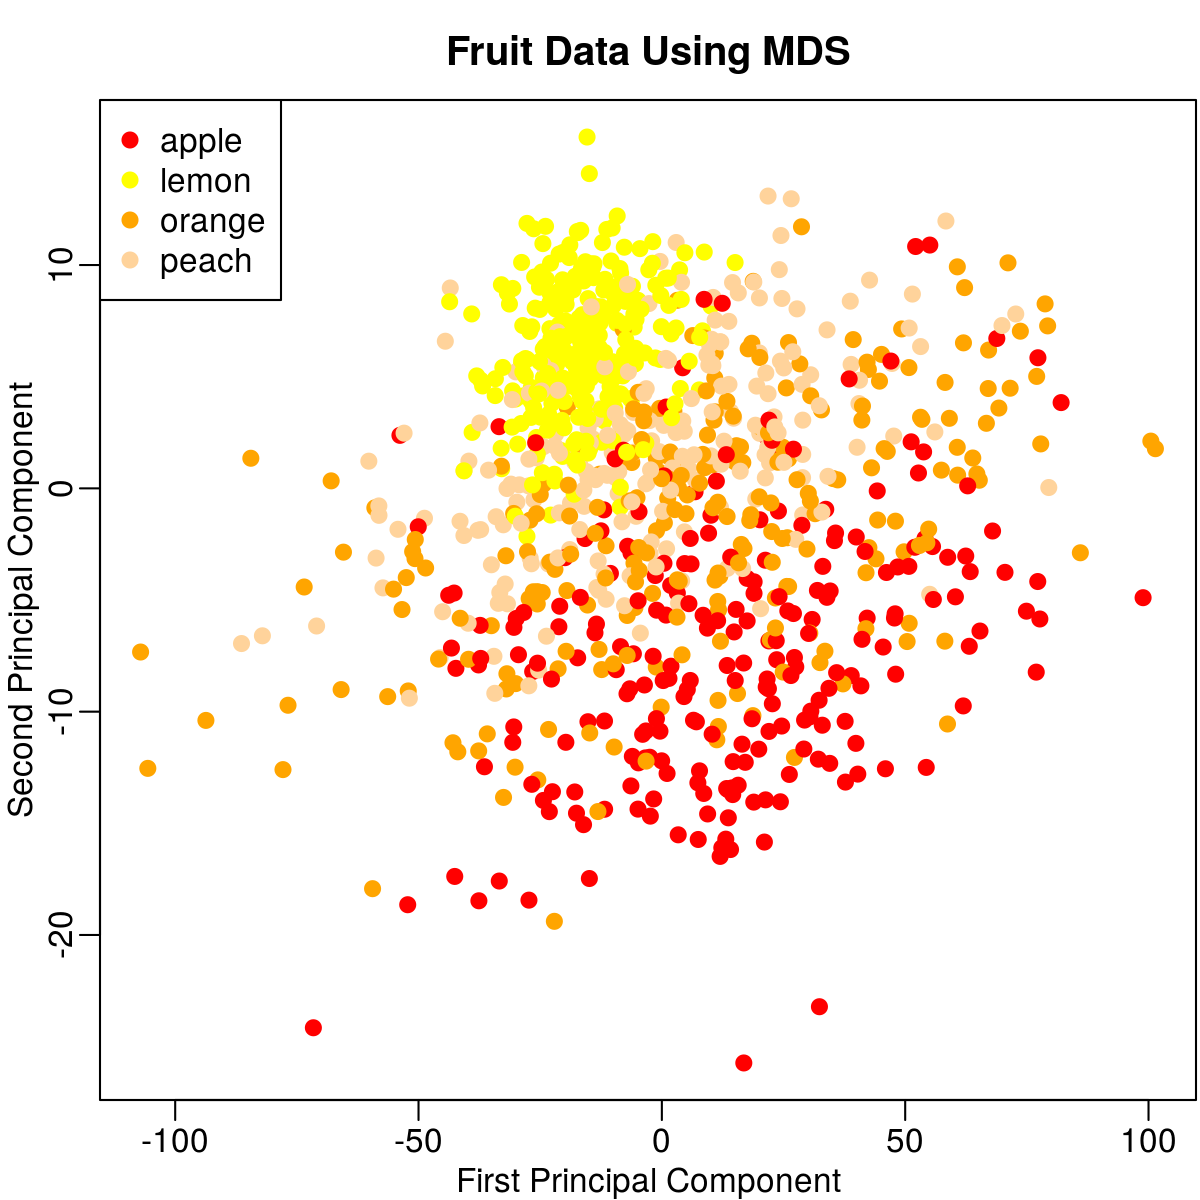
\includegraphics[width=0.45\textwidth]{images/mds_plot_fruit.png}
\end{figure}

\subsection{Source code :}

\begin{Rs}
# read the variable back in :
f = read.csv("../../data/fruit.csv")

# store the fruit 'classes' :
c = f[,5]

# store the fruit 'data' :
d = f[,seq(1,4)]

# perform MDS on d :
p = cmdscale(dist(d))

# store indexes of classes :
a = which(c == 'apple')
l = which(c == 'lemon')
o = which(c == 'orange')
z = which(c == 'peach')

# color vector :
cols  = c('red', 'yellow', 'orange', 'burlywood1')
cc    = as.vector(c)
cc[a] = cols[1]
cc[l] = cols[2]
cc[o] = cols[3]
cc[z] = cols[4]

# plot them colored by class :
png('../doc/images/mds_plot_fruit.png', res=200, width=6, height=6, units='in')
par(mar=c(2.5,2.5,2.5,.1),mgp = c(1.5, .5, 0))
plot(p, col=cc, bg=cc, type='p', pch=21, xlab='First Principal Component',
     ylab='Second Principal Component', main='Fruit Data Using MDS')
legend('topleft', levels(c), col = cols, pt.bg = cols, pch = 21)
dev.off()
\end{Rs}

\section{Mouse data :}

\begin{figure}[H]
  \centering
    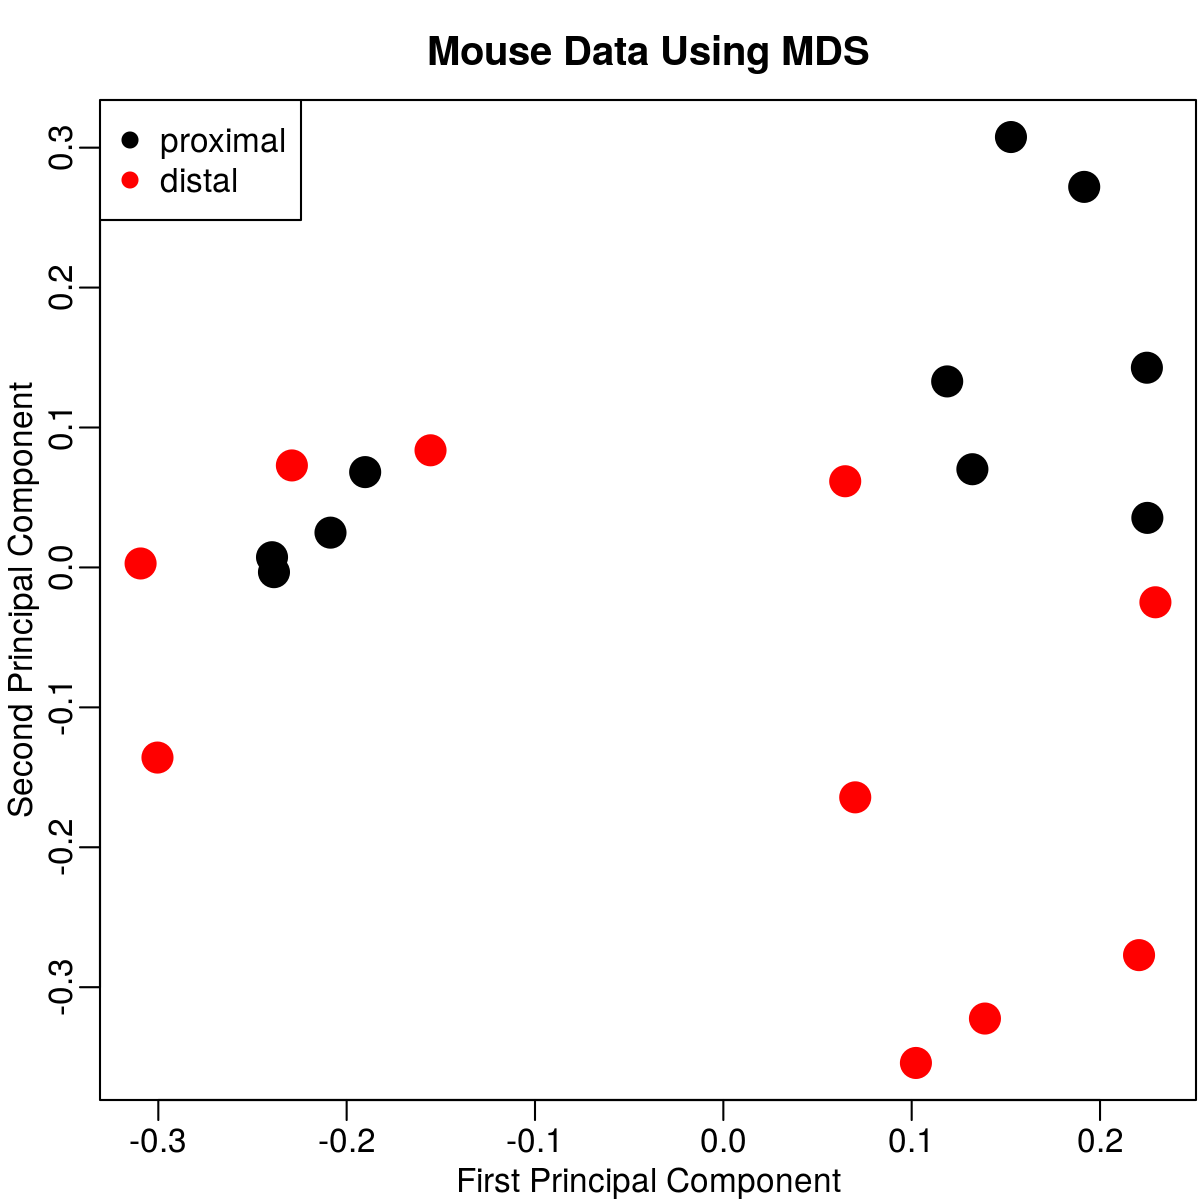
\includegraphics[width=0.45\textwidth]{images/mds_plot_mouse_experiment.png}
    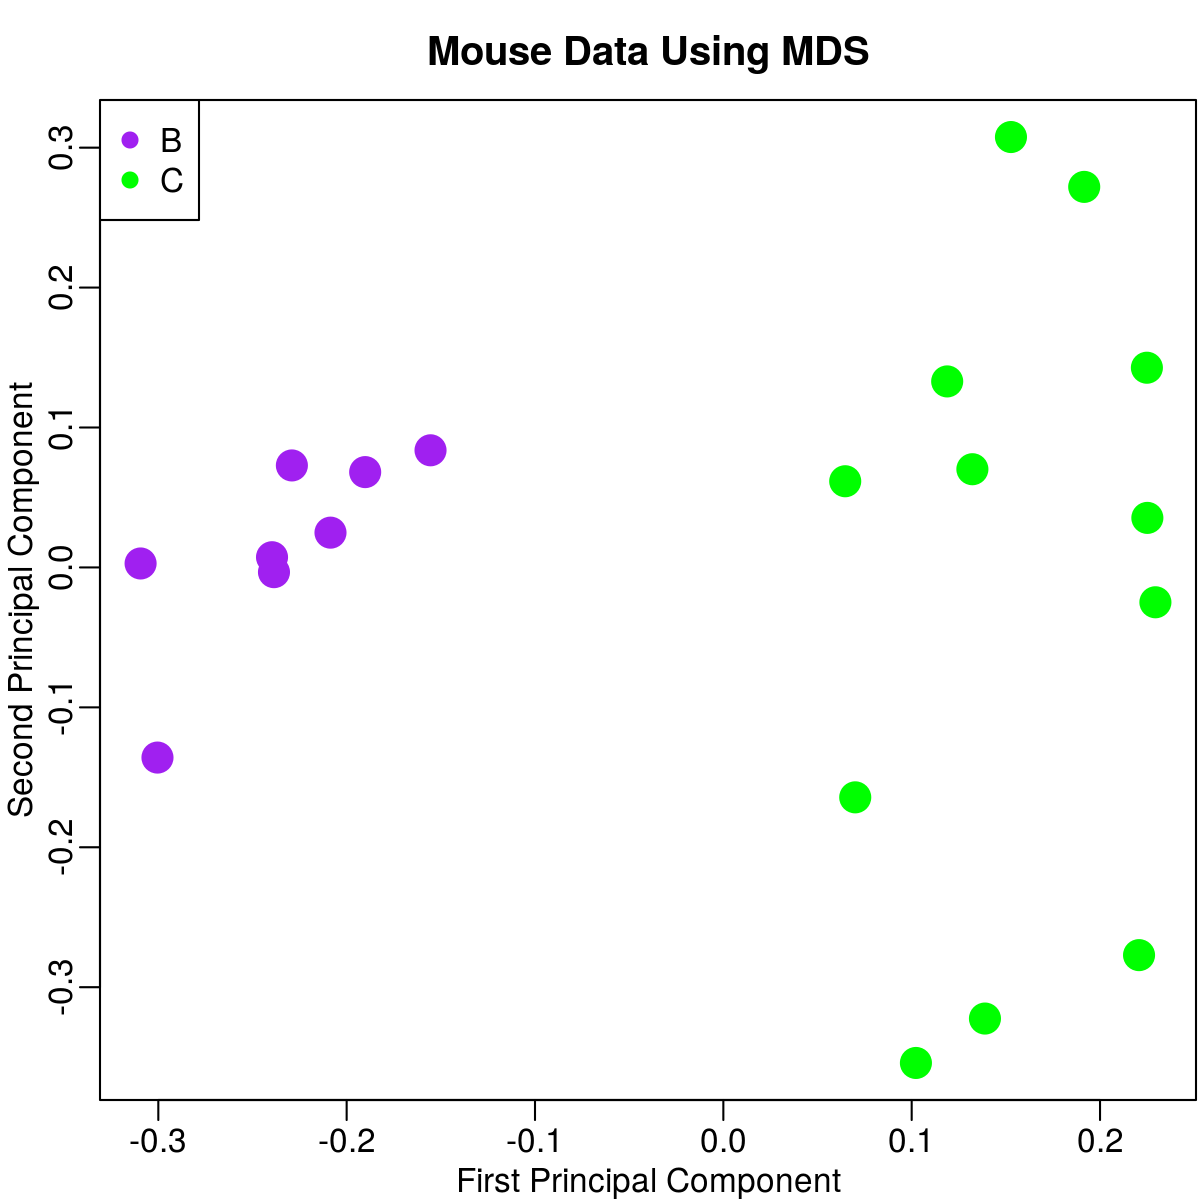
\includegraphics[width=0.45\textwidth]{images/mds_plot_mouse_type.png}
  \caption{MDS applied to the mouse data, showing a clustering by mouse type (bottom), rather than experiment type (top).}
\end{figure}

\subsection{Source code :}

\begin{Rs}
# read in the data :
f = read.csv("../../data/otu_table_L6.txt", sep="\t", row.names=1)

# get the experiment names :
e = colnames(f)

# store indexes of proximal (P) and distal (D) experiments, and mouse types
# B and C :
P = grep("[A-Z]+P[0-9]", e)
D = grep("[A-Z]+D[0-9]", e)
B = grep("^B[A-Z]+[0-9]", e)
C = grep("^C[A-Z]+[0-9]", e)

# transpose the data so each row is an experiment :
d = t(f)

# perform MDS on d :
p = cmdscale(dist(d))

# color vector :
cols  = c('black', 'red')
cc    = as.vector(e)
cc[P] = cols[1]
cc[D] = cols[2]

# plot them colored by experiment :
png('../doc/images/mds_plot_mouse_experiment.png', res=200, width=6, 
    height=6, units='in')
par(mar=c(2.5,2.5,2.5,.1),mgp = c(1.5, .5, 0))
plot(p, col=cc, bg=cc, type='p', pch=21, cex=2, 
     xlab='First Principal Component',
     ylab='Second Principal Component', main='Mouse Data Using MDS')
legend('topleft', c('proximal', 'distal'), col = cols, pt.bg = cols, pch = 21)
dev.off()

# color vector :
cols  = c('purple', 'green')
cc    = as.vector(e)
cc[B] = cols[1]
cc[C] = cols[2]

# plot them colored by mousey type :
png('../doc/images/mds_plot_mouse_type.png', res=200, width=6, 
    height=6, units='in')
par(mar=c(2.5,2.5,2.5,.1),mgp = c(1.5, .5, 0))
plot(p, col=cc, bg=cc, type='p', pch=21, cex=2,
     xlab='First Principal Component',
     ylab='Second Principal Component', main='Mouse Data Using MDS')
legend('topleft', c('B', 'C'), col = cols, pt.bg = cols, pch = 21)
dev.off()
\end{Rs}

\section{Tumors data :}

\begin{figure}[H]
  \centering
    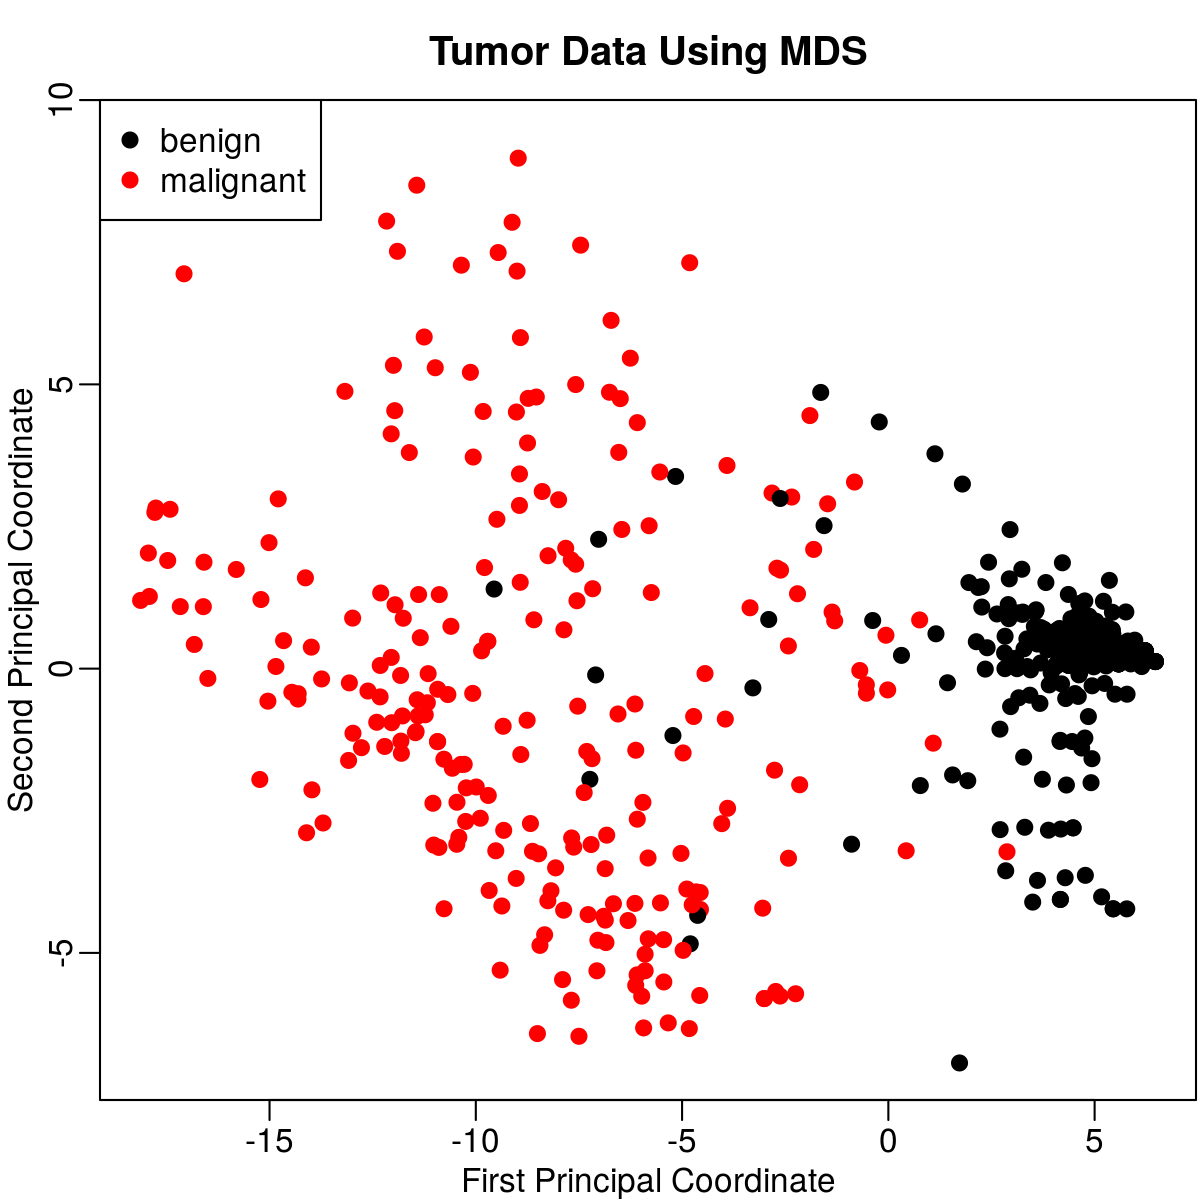
\includegraphics[width=0.45\textwidth]{images/mds_plot_tumor.png}
  \caption{MDS shows a clear separation between benign and malignant, with some overlap.}
\end{figure}

\subsection{Source code :}

\begin{Rs}
# read in the data :
f = read.csv("../../data/breast-cancer-wisconsin.data", header=FALSE)

# get the sample names :
e = f[,1]

# get the classes :
c = f[,11]

# get just the data :
d = f[,seq(2,10)]

# perform MDS on d :
p = cmdscale(dist(d))

# color sample black for benign (b) and red for malignant (m) :
cols  = c('black', 'red')
cc    = as.vector(e)
b     = which(c == 2)
m     = which(c == 4)
cc[b] = cols[1]
cc[m] = cols[2]

# plot them colored by experiment :
png('../doc/images/mds_plot_tumor.png', res=200, width=6, 
    height=6, units='in')
par(mar=c(2.5,2.5,2.5,.1),mgp = c(1.5, .5, 0))
plot(p, col=cc, bg=cc, type='p', pch=21, cex=1, 
     xlab='First Principal Coordinate',
     ylab='Second Principal Coordinate', main='Tumor Data Using MDS')
legend('topleft', c('benign', 'malignant'), col = cols, pt.bg = cols, pch = 21)
dev.off()
\end{Rs}

\end{multicols*}

%\begin{figure}[H]
%  \centering
%    \includegraphics[width=0.45\textwidth]{images/.png}
%\end{figure}


\end{document}


